\clearpage
\section{Why twenty-six rows, and what the other networks say}

T3 is not the corpus. It is a selection from it, made by two rules, and only one of them is
defensible. This section prints the funnel, names both rules, and measures what the selection did
to the numbers the table reports.

\subsection{The funnel, under the recovering set}

\begin{center}\small
\begin{tabular}{@{}rp{11.9cm}@{}}
\toprule
& stage \\
\midrule
39 & networks parsed from the corpus \\
33 & have a frame, meaning at least one treatment beside an undirected edge with the outcome a
possible descendant \\
27 & are swept. The six that are not exceed 500 nodes, or all their chain components exceed the
questionnaire cap \\
80{,}132 & candidate treatment--outcome pairs, built from observables alone \\
648 & pairs sampled into the frame, capped at twenty per network \\
537 & rows under the recovering set: 528 sampled plus 9 the source papers declare. All are
certifiable \\
234 & of those say the outcome cannot descend from the treatment on the analyst's own graph, so
the effect is zero and there is no adjustment set to report on \\
\textbf{303} & \textbf{commit to an adjustment set. This is the population a sensitivity report
could be written for: 9 declared and 294 sampled, over 27 networks} \\
\midrule
26 & are printed in T3 \\
\bottomrule
\end{tabular}
\end{center}

So the table shows 9 of the 9 declared queries and 17 of the 294 sampled ones, which is 5.8\,\% of
the eligible population. The 277 that are missing are missing for two different reasons.

\subsection{Rule one: only four networks have real coefficients}

Of the 27 swept networks, four carry coefficients fitted to real data: \texttt{ecoli70},
\texttt{arth150}, \texttt{magic-niab} and \texttt{magic-irri}. The other 23 carry structure from a
published source and parameters we drew ourselves, uniform in a fixed range with unit noise.

A sensitivity report on a named analysis prints an effect size and an interval. On a
semi-synthetic network those numbers are ours, not the field's, so the row would read as a report
on a real analysis while carrying an invented effect. That is why the other 23 networks contribute
257 eligible rows and none of them appear.

This rule is defensible and it should be printed in the caption, which it currently is not. Those
23 networks are not absent from the paper: they are the population behind the price table, the
certificate ladder and the funnel, where only the structure matters and the parameters are a
nuisance. They are absent from this one table, because this one table is about named effects.

\subsection{Rule two: the first five per network, and it is not defensible as written}

On the four remaining networks, 37 queries commit to a set and are therefore eligible. The table
takes five per network, which is 17 of 37, because \texttt{arth150} only has two.

The 20 that were dropped are 9 on \texttt{magic-niab}, 8 on \texttt{magic-irri} and 3 on
\texttt{ecoli70}. The cap is arbitrary and a reviewer will say so, but the cap is not the problem.
The ordering is.

\begin{verdict}
The eligible queries are sorted so that those with a finite null radius come first, and then the
first five are taken. A finite null radius means the interval reaches zero within the search depth,
which is the outcome the table exists to illustrate.

The effect is measurable. Across the 37 eligible queries, 16 have a finite null radius, which is
43\,\%. Among the 17 the table prints, 13 do, which is 76\,\%. Among the 20 it drops, 3 do, which
is 15\,\%.
\end{verdict}

So the null-radius column of T3 is not representative of the population it is drawn from, and the
fix is one line: sort by frame index alone, or print all 37. Either is honest and the second is
better, because the inclusion rule then has nothing in it that a reader has to trust.

\subsection{What the selection did not do}

The claim the figure of the previous section is built on survives the audit, and it survives it
comfortably.

\begin{center}\small
\begin{tabular}{@{}lccc@{}}
\toprule
population & queries & informative & of those, one retraction reaches the whole class \\
\midrule
printed in T3 & 17 & 16 & 16 of 16 \\
dropped by the cap & 20 & 10 & 10 of 10 \\
the full eligible pool & 37 & 26 & 26 of 26 \\
every committed row, 27 networks & 294 & 226 & 211 of 226 \\
\bottomrule
\end{tabular}
\end{center}

On every query the table could have shown, and on 93\,\% of every query in the corpus, retracting a
single claim returns the interval to the one the analyst would have had with no background knowledge
at all. The cap did not manufacture that pattern; it is the pattern of the corpus.

\begin{figure}[p]
\centering
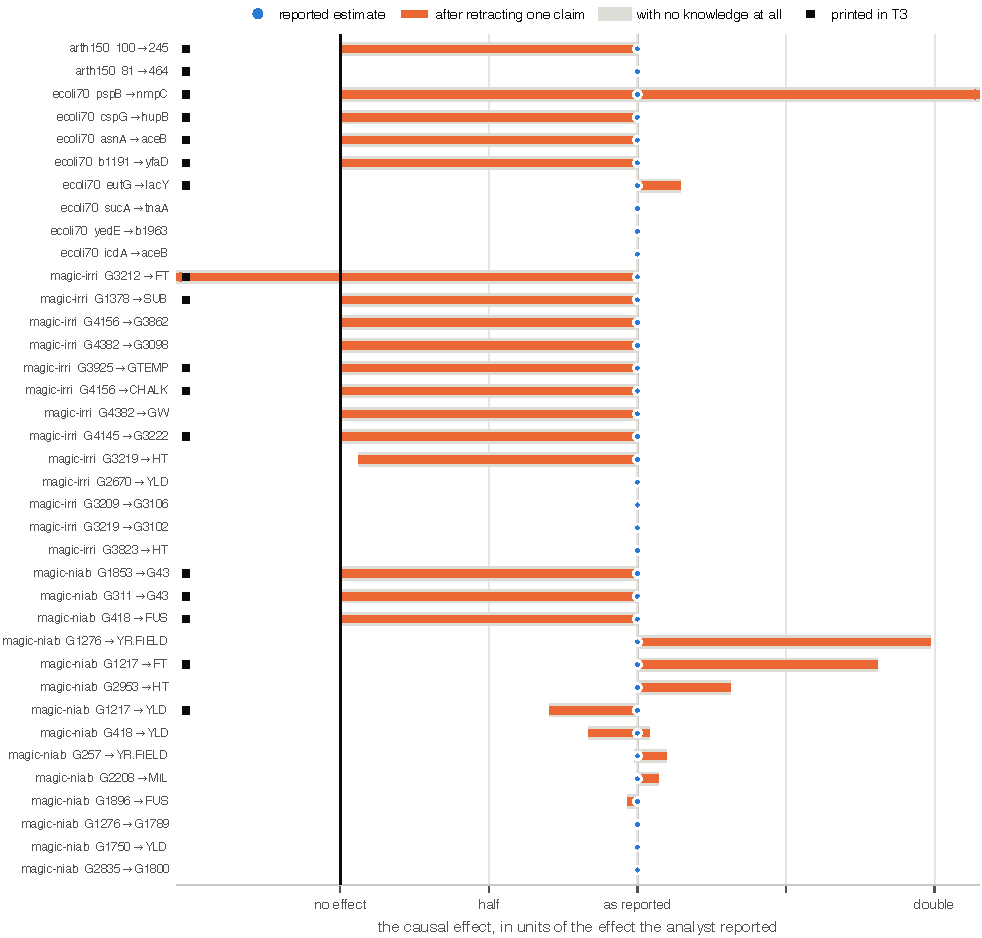
\includegraphics[width=\textwidth]{figs/f11_pool_dumbbell.pdf}
\caption{The recommended figure drawn on all 37 eligible queries rather than the seventeen T3
prints, with the printed ones marked. Eleven rows carry no bar at all: on those the class already
pins the effect and no retraction moves it, which is the honest counterweight and is invisible in
the table as printed.}
\end{figure}

\subsection{What to change}

Three things, and none of them is expensive.

Print the inclusion rule in T3's caption, naming both the real-coefficient restriction and the cap,
and give the count of eligible queries beside the count shown. Instance selection is this form's
whole attack surface and the only defence is stating the rule.

Remove the finite-null-radius term from the sort. The cap can stay at five per network if space
demands it, but taking the first five in frame order costs nothing and removes the bias from the
null-radius column.

Draw the figure on the 37, not the 17. It is the same picture, it is one page, it needs no
inclusion rule at all beyond the real-coefficient restriction, and it contains the eleven rows where
nothing moves, which the table currently hides.
